\documentclass[a4paper,12pt]{report}
\usepackage{a4wide}

%\documentclass[a5paper,10pt]{book}
%\usepackage[top=23mm, bottom=18mm, left=15mm, right=25mm]{geometry}
%\geometry{papersize={170mm,220mm}}


\usepackage[utf8x]{inputenc}
\usepackage[danish]{babel}

\usepackage{xr-hyper} %Externe hyper-ref
\usepackage[colorlinks=true, hyperindex=true, linkcolor=minmblaa, citecolor=minmblaa, urlcolor=minmblaa]{hyperref}
\hypersetup{colorlinks=true,filecolor=minmblaa,bookmarksnumbered=true} %Til hyperreferencer. Referencer med farver
\usepackage{needspace} % giver mulighed for at kræve at der skal være et antal tomme linier på siden før ellers indsættes et sideskift.
\usepackage{framed} %Bokse
\usepackage{wrapfig}

\usepackage{amsmath,amsfonts,amssymb,amsthm,mathtools} %Matematikpakker

\setlength{\parindent}{0mm} %Ingen Indhak i første linje i afsnit

\usepackage{color} %Farvepakke

\usepackage{array}
\usepackage{colortbl}
\usepackage{multirow} %Til at flette rækker i tabeller.

\usepackage{verbatim,mhchem}



	% DOWNLOAD FRA: http://sarovar.org/frs/?group_id=52&release_id=97
	% Læg i directory for hoved TEX fil
%\usepackage[draft]{pdfdraftcopy}
%\draftstring{Licens: Kasper Langt Mellemnavn Skårhøj}
%\draftfontsize{30}
	%\draftfontfamily{hlh}
	%\draftangle{45}
	%\definecolor{mycolor}{rgb}{.825,.855,1}
	%\draftcolor{mycolor}
	%\draftfontattrib



% = Sidehoved =
\usepackage{fancyhdr}
\pagestyle{fancy}
\renewcommand{\sectionmark}[1]{\markright{\protect\titlegraphic{dturoed}\textcolor{dtugraa}{\thesection~\MakeUppercase{#1}}}} % \thesection.\
\fancyhead{}
\fancyfoot{}
\fancyhead[R]{\titlefont\thepage}
\fancyhead[C]{}
\fancyhead[L]{\titlefont \small eNote \MakeUppercase{~\thechapter}~\hspace*{1ex}\rightmark}
\renewcommand\headrulewidth{0pt}
\fancypagestyle{plain}{\fancyfoot[C]{}}% {\titlefont\footnotesize\thepage}}
\setlength{\headheight}{15pt}


% = Længder
%\newlength{\envtblsep}\setlength{\envtblsep}{1\FrameSep}
\newlength{\obsl}\setlength{\obsl}{\textwidth-1.2cm-13.2pt}

% Includes:

% =     Fonts (select one)    =
\usepackage{mathpazo}\linespread{1.05} % Palatino needs more leading (space between lines)
\usepackage{bm} % bold math, must be loaded after the fontpackages

% % Til overskrifter
\DeclareTextFontCommand{\th}{\fontencoding{T1}\fontfamily{phv}\fontseries{b}\selectfont}
\newcommand\titlefont{\fontencoding{T1}\fontfamily{phv}\selectfont}


% =     PGF grafik      =
\usepackage{tikz}
\newcommand\titlegraphic[1]{%
\tikz[baseline] %
\draw[thick,color=#1]
(0pt  ,-0.25em) -- (0pt  ,0.85em)
(2.5pt,-0.25em) -- (2.5pt,0.85em)
(5pt  ,-0.25em) -- (5pt  ,0.85em)
(7.5pt,-0.25em) -- (7.5pt,0.85em);\hspace*{0.8ex} %
}

\newcommand\titlegraphicwide[1]{%
\tikz[baseline] %
\draw[line width=0.8mm,color=#1]
(0pt  ,-0.25em) -- (0pt  ,0.85em)
(4.5pt,-0.25em) -- (4.5pt,0.85em)
(9pt  ,-0.25em) -- (9pt  ,0.85em)
(13.5pt,-0.25em) -- (13.5pt,0.85em);\hspace*{0.8ex} %
}


% =      Title Layout      =
\usepackage{titlesec}
\makeatletter
\titleformat{\chapter}
	[display] % Shape
	{\titlefont\Huge\flushleft} % Title and label format
	{\titlefont\LARGE\bfseries \titlegraphicwide{dturoed}\textcolor{dtugraa}{\@chapapp~\thechapter}} % label
	{0.9em} % label/title separation
	{} % before code
	[] % after code
\makeatother
\titleformat{\section}
	[hang] % Shape
	{\titlefont\Large\flushleft} % Title and label format
	{\thesection} % label
	{0.9em} % label/title separation
	{} % before code
	[] % after code
\titleformat{\subsection}
	[hang] % Shape
	{\titlefont\large} % Title and label format
	{\thesubsection} % label
	{0.9em} % label/title separation
	{} % before code
	[] % after code
\titlespacing{\subsection}{0pt}{*6}{*1.5}
\titleformat{\subsubsection}
	[hang] % Shape
	{\titlefont} % Title and label format
	{\thesubsubsection} % label
	{0.9em} % label/title separation
	{} % before code
	[] % after code



% = Farver
\definecolor{dturoed}{rgb}{0.6, 0.0, 0.0}
\definecolor{dtugraa}{rgb}{0.5, 0.5, 0.5}	% Lidt mørkere. Korrekt = 0.4
\definecolor{mingroenstreg}{rgb}{0.4,0.8,0}	% Sekundærfarve 14 : 102/204/0	(Forårsgrøn) -> Eksempler
\definecolor{mingroen}{rgb}{0.32,0.64,0}		% Sekundærfarve 14, 80% mørkere (tekst)
\definecolor{minorangestreg}{rgb}{1,0.6,0}		% Sekundærfarve 1 : 255/153/0	(Orange) -> Opgaver
\definecolor{minorange}{rgb}{0.8,0.48,0}		% Sekundærfarve 1 , 80% mørkere (tekst)

\definecolor{minblaa}{rgb}{0.2,0.4,0.8}	% Sekundærfarve 13 , 51/102/204 	( Blå -> Definitioner etc)
\definecolor{minmblaa}{rgb}{0.16,0.32,0.64}	% Sekundærfarve 13 , 80% mørkere (tekst)
\definecolor{thmbackground}{rgb}{0.97,.97, 0.99}	% Farve 13 - lys baggrund

\definecolor{mingraastreg}{rgb}{.5,.5,.5}
\definecolor{hvadbackground}{rgb}{0.97,.97, 0.97}
\definecolor{sumgul}{rgb}{1,1,.8}

\definecolor{hjmopgfarve}{rgb}{.96,1,.96}


% = Counter
\newcounter{evncount}[chapter]
\setcounter{evncount}{0}
\renewcommand{\theevncount}{\thechapter.\arabic{evncount}}
\renewcommand{\theequation}{\thechapter-\arabic{equation}}


% = Eksempler = example =
\newenvironment{example}[1][]{
	\refstepcounter{evncount}
	\setlength{\obsl}{\textwidth-1.2cm-13.2pt-9pt} % fix width of the info envirnment%
	\def\FrameCommand{ 
		\textcolor{mingroenstreg}{\vrule width 4pt} 
		\hspace{5pt} 
	}%
	\MakeFramed{\advance\hsize-\width \FrameRestore}%
	\needspace{3\baselineskip}
	\titlegraphic{mingroen}
	\textcolor{mingroen}{
		\th{Eksempel \theevncount \hspace*{5mm} #1}
	} 
	\vspace*{3mm}%
	\begin{small}
	\par
}
{
	\end{small}
	\endMakeFramed
}


% = Opgaver = exercise =
\newenvironment{exercise}[1][]{
	\refstepcounter{evncount}
	\setlength{\obsl}{\textwidth-1.2cm-13.2pt-9pt}% fix width of the info envirnment%
	\def\FrameCommand{
		\textcolor{minorangestreg}{\vrule width 4pt}
		\hspace{5pt}
	}%
	\MakeFramed{\advance\hsize-\width \FrameRestore}%
	\needspace{3\baselineskip}
	\titlegraphic{minorange}
	\textcolor{minorange}{
		\th{Opgave \theevncount \hspace*{5mm} #1}
	} 
	\vspace*{3mm}%
	\begin{small}
	\par
}
{
	\end{small}
	\endMakeFramed
}


% = Bevis
\newenvironment{bevis}{
	\setlength{\obsl}{\textwidth-1.2cm-13.2pt-9pt} % fix width of the info envirnment%
	\def\FrameCommand{
		\textcolor{mingraastreg}{\vrule width 4pt} 
		\hspace{5pt}
	}%
	\MakeFramed{\advance\hsize-\width \FrameRestore}%
	\needspace{3\baselineskip}
	\titlegraphic{black}
	\textcolor{black}{
		\th{Bevis}
	}
	\vspace*{3mm}%
	\begin{small}
	\par
}
{
	\bevisslut 
	\end{small}
	\endMakeFramed
}


% = Definition =
\newenvironment{definition}[1][]{
	\vspace{4mm}
	\pagebreak[1]
	\setlength{\obsl}{\textwidth-1.2cm-2\FrameSep-13.2pt}%
	\def\FrameCommand{
		\fboxsep=\FrameSep\fcolorbox{minblaa}{thmbackground}
	}
	\begin{minipage}{\textwidth}
	\MakeFramed{\advance\hsize-\width\FrameRestore}
	\refstepcounter{evncount}
	\titlegraphic{minblaa}
	\textcolor{minmblaa}{
		\th{Definition \theevncount \hspace*{5mm} #1}
	}
	\vspace*{3mm}
	\par
}
{
	\endMakeFramed 
	\end{minipage}
	\vspace{4mm}
}


% = Theorem =
\newenvironment{theorem}[1][]{
	\vspace{4mm}
	\pagebreak[1]%
	\setlength{\obsl}{\textwidth-1.2cm-2\FrameSep-13.2pt}%
	\def\FrameCommand{
		\fboxsep=\FrameSep\fcolorbox{minblaa}{thmbackground}
	}%
	\begin{minipage}{\textwidth}
	\MakeFramed{\advance\hsize-\width\FrameRestore}%
	\refstepcounter{evncount}
	\titlegraphic{minblaa}
	\textcolor{minmblaa}{
		\th{Sætning \theevncount \hspace*{5mm} #1}
	}
	\vspace*{3mm}
	\par
}
{
	\endMakeFramed 
	\end{minipage}
	\vspace{4mm}
}


% = Lemma =
\newenvironment{lemma}[1][]{
	\vspace{4mm}
	\pagebreak[1]
	\setlength{\obsl}{\textwidth-1.2cm-2\FrameSep-13.2pt}%
	\def\FrameCommand{
		\fboxsep=\FrameSep \fcolorbox{minblaa}{thmbackground}
	}
	\begin{minipage}{\textwidth} 
	\MakeFramed{\advance\hsize-\width \FrameRestore}
	\refstepcounter{evncount}
	\titlegraphic{minblaa}
	\textcolor{minmblaa}{
		\th{Hjælpesætning \theevncount \hspace*{5mm} #1}
	}
	\vspace*{3mm}
	\par
}
{
	\endMakeFramed 
	\end{minipage}
	\vspace{4mm}
}


% = Corollary =
\newenvironment{corollary}[1][]{
	\vspace{4mm}
	\pagebreak[1]
	\setlength{\obsl}{\textwidth-1.2cm-2\FrameSep-13.2pt}%
	\def\FrameCommand{
		\fboxsep=\FrameSep \fcolorbox{minblaa}{thmbackground}
	}
	\begin{minipage}{\textwidth} 
	\MakeFramed{\advance\hsize-\width \FrameRestore}
	\refstepcounter{evncount}
	\titlegraphic{minblaa}
	\textcolor{minmblaa}{
		\th{Følgesætning \theevncount \hspace*{5mm} #1}
	}
	\vspace*{3mm}
	\par
}
{
	\endMakeFramed 
	\end{minipage}
	\vspace{4mm}
}


% = Metode = method
\newenvironment{method}[1][]{
	\vspace{4mm}
	\pagebreak[1]
	\setlength{\obsl}{\textwidth-1.2cm-2\FrameSep-13.2pt}%
	\def\FrameCommand{
		\fboxsep=\FrameSep \fcolorbox{black}{hvadbackground}
	}
	\begin{minipage}{\textwidth} 
	\MakeFramed{\advance\hsize-\width \FrameRestore}
	\refstepcounter{evncount}
	\titlegraphic{black}
	\textcolor{black}{
		\th{Metode \theevncount \hspace*{5mm} #1}
	}
	\vspace*{3mm}
	\par
}
{
	\endMakeFramed
	\end{minipage}
	\vspace{4mm}
}


% = Forklaring = explain =
\newenvironment{explain}[1][]{
	\vspace{4mm}
	\pagebreak[1]
	\setlength{\obsl}{\textwidth-1.2cm-2\FrameSep-13.2pt}%
	\def\FrameCommand{
		\fboxsep=\FrameSep \fcolorbox{black}{hvadbackground}
	}
	\MakeFramed{\advance\hsize-\width \FrameRestore}
	\refstepcounter{evncount}
	\titlegraphic{black}
	\textcolor{black}{
		\th{Forklaring \theevncount \hspace*{5mm} #1}
	}
	\vspace*{3mm}
	\par
}
{
	\endMakeFramed
	\vspace{4mm}
}


% = Bemærkning = remark =
\newenvironment{remark}[1][]{
	\vspace{4mm}
	\pagebreak[1]
	\setlength{\obsl}{\textwidth-1.2cm-2\FrameSep-13.2pt}%
	\def\FrameCommand{
		\fboxsep=\FrameSep \fcolorbox{black}{hvadbackground}
	}
	\begin{minipage}{\textwidth} 
	\MakeFramed{\advance\hsize-\width \FrameRestore}
	\refstepcounter{evncount}
	\titlegraphic{black}
	\textcolor{black}{
		\th{Bemærkning \theevncount \hspace*{5mm} #1}
	}
	\vspace*{3mm}
	\par
}
{
	\endMakeFramed 
	\end{minipage}
	\vspace{4mm}
}







% = OBS! = obs =
\newenvironment{obs}{\vspace{4mm}\par%
\begin{tabular}{m{1.2cm}<{\hspace*{2mm}}@{}|m{\obsl}@{}}\hspace*{-4pt}\raggedleft
\includegraphics[width=1.1cm]{../Strukturfiler/FIGS/Alert01} & \begin{minipage}{\obsl}}{\end{minipage}\\ \end{tabular}\vspace{4mm}\par}


% = INFO = info =
\newenvironment{info}{\vspace{4mm}\par%
\begin{tabular}{m{1.2cm}<{\hspace*{2mm}}@{}|m{\obsl}@{}}\hspace*{-4pt}\raggedleft
\includegraphics[width=1.1cm]{../Strukturfiler/FIGS/Info01} & \begin{minipage}{\obsl}}{\end{minipage}\\ \end{tabular}\vspace{4mm}\par}


% = THINK= think =
\newenvironment{think}{\vspace{4mm}\par%
\begin{tabular}{m{1.2cm}<{\hspace*{2mm}}@{}|m{\obsl}@{}}\hspace*{-4pt}\raggedleft
\includegraphics[width=0.7cm]{../Strukturfiler/FIGS/ChessPiece} & \begin{minipage}{\obsl}}{\end{minipage}\\ \end{tabular}\vspace{4mm}\par}


% = AHA= aha =
\newenvironment{aha}{\vspace{4mm}\par%
\begin{tabular}{m{1.2cm}<{\hspace*{2mm}}@{}|m{\obsl}@{}}\hspace*{-4pt}\raggedleft
\includegraphics[width=1.1cm]{../Strukturfiler/FIGS/Think} & \begin{minipage}{\obsl}}{\end{minipage}\\ \end{tabular}\vspace{4mm}\par}


% = BUILDUP= build =
\newenvironment{build}{\vspace{4mm}\par%
\begin{tabular}{m{1.2cm}<{\hspace*{2mm}}@{}|m{\obsl}@{}}\hspace*{-4pt}\raggedleft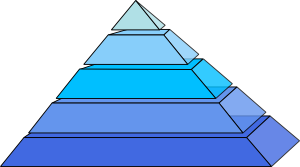
\includegraphics[width=1.1cm]{../Strukturfiler/FIGS/BluePyramid} & \begin{minipage}{\obsl}}{\end{minipage}\\ \end{tabular}\vspace{4mm}\newline}


% = Forudsætning = basis
\newenvironment{basis}{\begin{flushleft} \begin{itshape} }{\end{itshape} \end{flushleft}}


% = Opsummering =
\newenvironment{summary}{\clearpage\pagecolor{sumgul}\section{Opsummering}}{\newpage\pagecolor{white}}











% = Counter
\newcounter{opgavecount}[section]
\setcounter{opgavecount}{0}
\newcounter{spgcount}[opgavecount]
\setcounter{spgcount}{0}
\renewcommand{\thespgcount}{\alph{spgcount})}



% = EXERCISE = (DIVIDER)

\newcommand{\exercisebegin}[1][]{\bigskip\needspace{3\baselineskip}\refstepcounter{opgavecount}\titlegraphic{mingroen}\textcolor{mingroen}{\th{Opgave \theopgavecount \hspace*{1cm} #1}}\medskip\par}

% = QUIZEXERCISE = (DIVIDER)

\newcommand{\quizexercisebegin}[1][]{\bigskip\needspace{3\baselineskip}\refstepcounter{opgavecount}\titlegraphic{mingroen}\textcolor{mingroen}{\th{Quiz-Opgave \theopgavecount \hspace*{1cm} #1}}\medskip\par}

% = QUESTION =

\newenvironment{question}{\refstepcounter{spgcount}\begin{itemize}\item[\thespgcount]}{\end{itemize}\hspace*{\fill}}

% = VINK =

\newenvironment{vink}{\begin{tabular}{m{.9cm}<{\hspace*{2mm}}@{}|m{\obsl}@{}}\hspace*{-4pt}\raggedleft
\includegraphics[width=.9cm]{../Strukturfiler/FIGS/Think} & \begin{minipage}{\obsl}}{\end{minipage}\\ \end{tabular}\medskip\\}
	
% = FACIT =

\newenvironment{facit}{\begin{tabular}{m{.9cm}<{\hspace*{2mm}}@{}|m{\obsl}@{}}\hspace*{-4pt}\raggedleft
\includegraphics[width=.9cm]{../Strukturfiler/FIGS/Check} & \begin{minipage}{\obsl}}{\end{minipage}\\ \end{tabular}\medskip\\}








\newcommand{\afsnit}[1]{\bigskip\th{\titlegraphic{mingroen}\textcolor{mingroen}{#1}} \\ \rule[7pt]{.4\textwidth}{1pt} \vspace*{-2.5mm}\par}

% (DIVIDER):
\newcommand{\ugedagdatotitel}[4]{\pagebreak[4]\section{Semesteruge #1 -- #2 Dag \hspace*{1mm} (#3)} \vspace*{-4mm} \rule[5pt]{\textwidth}{1pt}\vspace*{-2.5mm} \begin{center}\large{\th{#4}}\end{center} \fancyhead[C]{\th{Semesteruge #1}}}

\newenvironment{skema}[1]{\definecolor{shadecolor}{rgb}{0.96,.98, 1.0} \setlength{\FrameSep}{6pt} \renewcommand{\FrameHeightAdjust}{10pt} \vspace*{-4pt}\begin{shaded} \begin{tabular}{#1}}{\end{tabular} \end{shaded} \vspace*{-7pt}}


% ========================

% MAKROER

%\newenvironment{matr}[1][]{\hspace*{-.8mm}\left[\hspace*{-1mm}\begin{array}{#1}}{\end{array}\hspace*{-1mm}\right]\hspace*{-.8mm}}
\newcommand{\bevisslut}{\begin{scriptsize} \begin{flushright} $ \blacksquare $ \end{flushright} \end{scriptsize}}

\newcommand{\tref}[2]{\hyperref[#1]{#2 \ref*{#1}}}
\newcommand{\thref}[2]{\hyperref[#1]{#2}}

\newcommand{\refA}[1]{\colorbox{yellow}{\ref{#1}}}
\newcommand{\hrefA}[2]{\colorbox{yellow}{\href{#1}{#2}}}
\newcommand{\trefA}[2]{\colorbox{yellow}{\hyperref[#1]{#2 \ref*{#1}}}}
\newcommand{\threfA}[2]{\colorbox{yellow}{\hyperref[#1]{#2}}}

\newenvironment{matr}[1]{\hspace*{-.8mm}\begin{bmatrix}\hspace*{-1mm}\begin{array}{#1}}{\end{array}\hspace*{-1mm}\end{bmatrix}\hspace*{-.8mm}}
\newcommand{\transp}{\hspace*{-.6mm}^{\top}}

\newcommand{\maengde}[2]{\left\lbrace \hspace*{-1mm} \begin{array}{c|c} #1 & #2 \end{array} \hspace*{-1mm} \right\rbrace}

\newenvironment{eqnalign}[1]{\setlength{\arraycolsep}{1.3pt}\begin{equation}\begin{array}{#1}}{\end{array}\end{equation}\par}
\newcommand{\eqnl}{\setlength{\arraycolsep}{1.3pt}}

\newcommand{\matind}[3]{{_\mathrm{#1}\mathbf{#2}_\mathrm{#3}}}
\newcommand{\vekind}[2]{{_\mathrm{#1}\mathbf{#2}}}
\newcommand{\jac}[2]{{\mathrm{Jacobi}_\mathbf{#1} (#2)}}
\newcommand{\diver}[2]{{\mathrm{div}\mathbf{#1} (#2)}}
\newcommand{\rot}[1]{{\mathbf{rot}\mathbf{(#1)}}}

\newcommand{\am}{\mathrm{am}}
\newcommand{\gm}{\mathrm{gm}}
\newcommand{\E}{\mathrm{E}}
\newcommand{\Span}{\mathrm{span}}
\newcommand{\mU}{\mathbf{U}}

\newcommand{\ms}{\medskip\\}
\newcommand{\bs}{\bigskip\\}

\newcommand{\mA}{\mathbf{A}}
\newcommand{\mB}{\mathbf{B}}
\newcommand{\mC}{\mathbf{C}}
\newcommand{\mD}{\mathbf{D}}
\newcommand{\mE}{\mathbf{E}}
\newcommand{\mF}{\mathbf{F}}
\newcommand{\mK}{\mathbf{K}}
\newcommand{\mI}{\mathbf{I}}
\newcommand{\mM}{\mathbf{M}}
\newcommand{\mN}{\mathbf{N}}
\newcommand{\mQ}{\mathbf{Q}}
\newcommand{\mT}{\mathbf{T}}
\newcommand{\mV}{\mathbf{V}}
\newcommand{\mW}{\mathbf{W}}
\newcommand{\mX}{\mathbf{X}}
\newcommand{\ma}{\mathbf{a}}
\newcommand{\mb}{\mathbf{b}}
\newcommand{\mc}{\mathbf{c}}
\newcommand{\md}{\mathbf{d}}
\newcommand{\me}{\mathbf{e}}
\newcommand{\mn}{\mathbf{n}}
\newcommand{\mr}{\mathbf{r}}
\newcommand{\mv}{\mathbf{v}}
\newcommand{\mw}{\mathbf{w}}
\newcommand{\mx}{\mathbf{x}}
\newcommand{\mxb}{\mathbf{x_{bet}}}
\newcommand{\my}{\mathbf{y}}
\newcommand{\mz}{\mathbf{z}}
\newcommand{\reel}{\mathbb{R}}
\newcommand{\mL}{\bm{\Lambda}} %Lambda-matrix
\newcommand{\mnul}{\bm{0}}
\newcommand{\trap}[1]{\mathrm{trap}(#1)}
\newcommand{\Det}{\operatorname{Det}}
\newcommand{\adj}{\operatorname{adj}}
\newcommand{\Ar}{\operatorname{Areal}}
\newcommand{\Vol}{\operatorname{Vol}}
\newcommand{\Rum}{\operatorname{Rum}}
\newcommand{\diag}{\operatorname{\bf{diag}}}
\newcommand{\bidiag}{\operatorname{\bf{bidiag}}}
\newcommand{\spanVec}[1]{\mathrm{span}\{#1\}}
\newcommand{\Div}{\operatorname{Div}}
\newcommand{\Rot}{\operatorname{\mathbf{Rot}}}

\newcommand{\Jac}{\operatorname{Jacobi}}
\newcommand{\Tan}{\operatorname{Tan}}
\newcommand{\Ort}{\operatorname{Ort}}
\newcommand{\Flux}{\operatorname{Flux}}
\newcommand{\Cmass}{\operatorname{Cm}}
\newcommand{\Imom}{\operatorname{Im}}
\newcommand{\Pmom}{\operatorname{Pm}}
\newcommand{\IS}{\operatorname{I}}
\newcommand{\IIS}{\operatorname{II}}
\newcommand{\IIIS}{\operatorname{III}}
\newcommand{\Le}{\operatorname{L}}
\newcommand{\app}{\operatorname{app}}
\newcommand{\M}{\operatorname{M}}
\newcommand{\re}{\mathrm{Re}}
\newcommand{\im}{\mathrm{Im}}

\newcommand{\compl}{\mathbb{C}} %de komplekse tal
\newcommand{\e}{\mathrm{e}} %eksponentialfunktionen. lodret 'e', og altså ikke kursiv ligesom andre bogstaver.





% Medialink: SCREEN: (QRcode) + thumbnail image + link på kodenummer (til qr.dtu.dk)
\newcommand{\onlinemedia}[3]{
	\begin{wrapfigure}{r}{3.2cm} 
		\vspace{-30pt} 
		\vspace{#1pt} 
		\begin{flushright} 
			\includegraphics[width=3cm]{qr/#2.png} 
			\tiny 
			\href{http://qr.dtu.dk/#2}{#2: #3}
			\normalsize  
		\end{flushright} 
		\vspace{-10pt} 
	\end{wrapfigure}
}
\newcommand{\onlinemediathumb}[3]{
	\begin{wrapfigure}{r}{3.2cm} 
		\vspace{-30pt} 
		\vspace{#1pt} 
		\begin{flushright} 
			\includegraphics[width=3cm]{qr/#2.png} 
			\includegraphics[width=3cm]{qr/#2_thumb.png} 
			\tiny 
			\href{http://qr.dtu.dk/#2}{#2: #3}
			\normalsize  
		\end{flushright} 
		\vspace{-10pt} 
	\end{wrapfigure}
}



% Index:
\usepackage{makeidx}
\makeindex
\newcommand\ind[2]{\index{#1}\textbf{\textit{\textcolor{black}{#2}}}}

% ###SERVER_EXCLUDE_BEGIN###
\externaldocument[NUID17-]{../../enoten/TN01-Talrum/Talrum}
\externaldocument[NUID1-]{../../enoten/TN02-Ligningssystemer/TNdriver}
\externaldocument[NUID2-]{../../enoten/TN03-Matricer_og_Matrixalgebra/Matricer_og_matrixalgebra}
\externaldocument[NUID3-]{../../enoten/TN04-Kvadratiske_matricer/TNdriver}
\externaldocument[NUID11-]{../../enoten/TN05-Determinanter/Determinanter}
\externaldocument[NUID12-]{../../enoten/TN06-GeometriskeVektorer/GeometriskeVektorer}
\externaldocument[NUID18-]{../../enoten/TN07-Vektorrum/VektorRum}
\externaldocument[NUID21-]{../../enoten/TN08-LinAfbildninger/LinAfbildninger}
\externaldocument[NUID23-]{../../enoten/TN09-Egenvaerdier_og_egenvektorer/TNdriver}
\externaldocument[NUID24-]{../../enoten/TN10-Diagonalisering_med_egenvektorer/TNdriver}
\externaldocument[NUID10-]{../../enoten/TN11-1.ordens_differentialligninger/TNdriver}
\externaldocument[NUID13-]{../../enoten/TN12-1.ordens_differentialligningssystemer/TNdriver}
\externaldocument[NUID14-]{../../enoten/TN13-2.ordens_differentialligninger/TNdriver}
\externaldocument[NUID27-]{../../enoten/TN14-Elemenataere_funktioner/Elementaere_Funktioner}
\externaldocument[NUID28-]{../../enoten/TN15-Funktioner2Variable/Funktioner_To_Variable}
\externaldocument[NUID29-]{../../enoten/TN16-Gradienter_og_Tangentplaner/Gradienter_og_Tangentplaner}
\externaldocument[NUID32-]{../../enoten/TN17-Taylor_formler/Taylor_Formler}
\externaldocument[NUID33-]{../../enoten/TN18-Taylor_2Var/Taylor_2Var}
\externaldocument[NUID34-]{../../enoten/TN19-SymMat/SymmetriskeMatricer}
\externaldocument[NUID35-]{../../enoten/TN20-KegleSnit/Keglesnit}
\externaldocument[NUID36-]{../../enoten/TN21-Riemann_Integral/Riemann_01}
\externaldocument[NUID37-]{../../enoten/TN22-Plan_Int/Plan_Int_01}
\externaldocument[NUID39-]{../../enoten/TN23-Flade_Int/Flade_Rum_Int_01}
\externaldocument[NUID40-]{../../enoten/TN24-Vektorfelter/Vektorfelter_01}
\externaldocument[NUID41-]{../../enoten/TN25-Flux/Flux_02}
\externaldocument[NUID42-]{../../enoten/TN26-Gauss/Gauss_01}
\externaldocument[NUID128-]{../../enoten/TN27-Stokes/Stokes_01}
\externaldocument[NUID43-]{../../enoten/TN29-KomplekseTal/KomplekseTal}

\externaldocument[NUID6-]{../../E-math-opgaver/Opgaver/opgU123}
\externaldocument[NUID19-]{../../E-math-opgaver/Opgaver/opgU45}
\externaldocument[NUID20-]{../../E-math-opgaver/Opgaver/opgU678}
\externaldocument[NUID25-]{../../E-math-opgaver/Opgaver/opgU910SD}
\externaldocument[NUID31-]{../../E-math-opgaver/OpgaverF11-U123/opgF123}
% \externaldocument[NUID9-]{../../E-math-opgaver/Opgaver/Dagsordner E10}
% ###SERVER_EXCLUDE_END###


% Begin document and set alternative chapter title:
\begin{document}
\renewcommand{\chaptername}{eNote}

\setcounter{chapter}{12} %SÆT DETTE TAL TIL 1 MINDRE END DET AKTUELLE TRANSFERNOTE-NUMMER!!

%%%%%%%%%%%%%%%%%%%%%%%%%%%%%%%%%%%%%%%%%%%%%
%%%%%%%%%%%%%%%%%%%%%%%%%%%%%%%%%%%%%%%%%%%%%
%%% HERFRA SKAL DU SKRIVE ELLER INDSÆTTE %%%%
%%% DEN FIL DU ØNSKER %%%%%%%%%%%%%%%%%%%%%%%
%%%%%%%%%%%%%%%%%%%%%%%%%%%%%%%%%%%%%%%%%%%%%
%%%%%%%%%%%%%%%%%%%%%%%%%%%%%%%%%%%%%%%%%%%%%

\chapter[Lineære 2. ordens differentialligninger]{Lineære 2. ordens differentialligninger med konstante koefficienter} \label{tn13}

\begin{basis}
I forlængelse af \tref{NUID10-tn11}{eNote} og \tref{NUID13-tn12}{eNote} om differentialligninger, kommer nu denne eNote omkring 2. ordens differentialligninger. Dele af bevisførelser m.m. læner sig op af de foregående noter, hvorfor det forudsættes, at man har kendskab til dem. Endvidere benyttes de komplekse tal.
\end{basis}

I \tref{NUID13-subsek.omf1}{afsnit} i \tref{NUID13-tn12}{eNote} behandles $ n $-te ordens homogene differentialligninger. Denne note handler netop de lineære differentialligninger, hvor $ n = 2 $, hvorfor teorien kan overføres. Vi vil i denne note også behandle de \textit{inhomogene} 2. ordens differentialligninger, så teorien skal udvides. Lineære inhomogene 2. ordens differentialligninger med konstante koefficienter har følgende principielle udseende:
\begin{equation}
x''(t) + a_1x'(t) + a_0x(t) = q(t), \quad t \in I, q : I \rightarrow \reel
\end{equation}
$ a_0, a_1 \in \reel $ er konstante koefficienter til $ x(t) $ henholdsvis $ x'(t) $, og de er altså ikke funktioner af $ t $. $ q(t) $ kaldes højresiden og er en funktion af $ t $. At denne type differentialligning er lineær, er op til læseren at vise (for eksempel ved hjælp af \tref{NUID10-saet.lindiff1}{definition}). Fremgangsmåden til at løse en 2. ordens differentialligning foregår i to trin.

\begin{method}[Løsningens struktur] \label{saet.difflig2.struk1}
Den fuldstændige løsningsmængde $ L_{inhom} $ til den lineære 2. ordens differentialligning
\begin{equation}
x''(t) + a_1x'(t) + a_0x(t) = q(t), \quad t \in I, q : I \rightarrow \reel, \label{lig.saet.difflig2.struk1}
\end{equation}
hvor $ a_0, a_1 \in \reel $ er konstante koefficienter, kan ved hjælp af \tref{NUID10-saet.hovedstruktur1}{sætning} opdeles i to:
\begin{enumerate}
\item Den fuldstændige løsningsmængde $ L_{hom} $ til den tilsvarende homogene differentialligning, for eksempel bestemt ved sætning \ref{saet.difflig2.hom1}.
\item En partikulær løsning $ x_0(t) $ til den inhomogene differentialligning, for eksempel bestemt med et gæt. Se afsnit \ref{subsek.difflig2.inhom1}.
\end{enumerate}
Strukturen af løsningen er da
\begin{equation}
L_{inhom} = x_0(t) + L_{hom},
\end{equation}
som det også fremgår i \tref{NUID10-saet.hovedstruktur1}{sætning}.
\end{method}

Som det fremgår af metoden ovenfor kan man opsplitte løsningsproceduren i to. Hver af de to dele vil herunder blive beskrevet i de to nedenstående afsnit. Slutteligt behandles eksistens og entydighed. \bs
Eksempler på den fuldstændige løsningsmængde til den 2. ordens differentialligning kan findes sidst i noten (for eksempel eksempel \ref{eks.difflig2.eksent21}).

\section{Den homogene differentialligning} \label{subsek.difflig2.hom1}

Vi betragter nu den lineære homogene 2. ordens differentialligning med konstante koefficienter
\begin{equation}
x''(t) + a_1x'(t) + a_0x(t) = 0, \quad t \in \reel \,, a_0,a_1 \in \reel
\end{equation}
Vi ønsker at bestemme den fuldstændige løsningsmængde til denne, primært fordi den er en del af den inhomogene differentialligning, som ses i metode \ref{saet.difflig2.struk1}. Her kommer nogle helt klare løsningsformer alt efter ligningens udseende.

\begin{theorem}[Løsning til homogen] \label{saet.difflig2.hom1}
Den homogene differentialligning
\begin{equation}
x''(t) + a_1x'(t) + a_0x(t) = 0, \quad t \in \reel, \label{lig.difflig2.hom1}
\end{equation}
har den såkaldte \ind{karakterligning}{karakterligning}
\begin{equation}
\lambda^2 + a_1 \lambda + a_0 = 0.
\end{equation}
Typen af rødder til denne ligning afgør udseendet af den fuldstændige løsningsmængde $ L_{hom} $ til den homogene differentialligning.
\begin{itemize}
\item \textbf{To forskellige reelle rødder} $ \lambda_1 $ og $ \lambda_2 $ giver løsningen 
\begin{equation}
x(t) = c_1\e^{\lambda_1 t} + c_2\e^{\lambda_2 t}, \quad t \in \reel.
\end{equation}
\item \textbf{To komplekse rødder} $ \lambda = \alpha \pm \beta i $ giver den reelle løsning
\begin{equation} \label{lig.kompl1}
x(t) = c_1\e^{\alpha t}\cos(\beta t) + c_2\e^{\alpha t}\sin(\beta t), \quad t \in \reel.
\end{equation}
\item \textbf{Dobbeltroden} $ \lambda $ giver løsningen
\begin{equation}
x(t) = c_1\e^{\lambda t} + c_2 t \e^{\lambda t}, \quad t \in \reel.
\end{equation}
\end{itemize}
For alle tre tilfælde gælder, at de respektive funktioner for alle $ c_1,c_2 \in \reel $ udgør den fuldstændige løsningsmængde $ L_{hom} $.
\end{theorem}

\begin{info}
I \tref{NUID13-subsek.omf1}{afsnit} gennemgås teorien for at omforme netop denne type differentialligning til et system af 1. ordens differentialligninger. Det er en absolut brugbar løsning. Systemet vil da se således ud:
\begin{equation}
\begin{matr}{c} x_1'(t) \\ x_2'(t) \end{matr} = \begin{matr}{cc} 0 & 1 \\ -a_0 & -a_1 \end{matr} \begin{matr}{c} x_1(t) \\ x_2(t) \end{matr}
\end{equation}
hvor $ x_1(t) = x(t) $ og $ x_2(t) = x_1'(t) = x'(t) $. Vi kan i så fald bruge den gennemgåede teori til at løse problemet.
\end{info}

\begin{bevis} \label{bed.difflig2.hom21}
Den homogene 2. ordens lineære differentialligning \eqref{lig.difflig2.hom1} omformes et 1. ordens differentialligningsystem:
\begin{equation}
\begin{matr}{c} x_1'(t) \\ x_2'(t) \end{matr} = \begin{matr}{cc} 0 & 1 \\ -a_0 & -a_1 \end{matr} \begin{matr}{c} x_1(t) \\ x_2(t) \end{matr} = \mA \begin{matr}{c} x_1(t) \\ x_2(t) \end{matr}
\end{equation}
hvor $ x_1(t) = x(t) $ er den søgte løsning, som udgør den fuldstændige løsningsmængde. Bevisførelsen tager udgangspunkt i sætningerne og metoderne i \tref{NUID13-sek.diffsys.struktur1}{afsnit}. Til det skal man bruge egenværdierne til systemmatricen $ \mA $:
\begin{equation}
\mathrm{det}(\mA - \lambda \mE) = \begin{vmatrix} -\lambda & 1 \\ -a_0 & -a_1-\lambda \end{vmatrix} = \lambda^2 + a_1\lambda + a_0 = 0,
\end{equation}
hvilket netop er karakterligningen tilhørende differentialligningen, og $ \lambda $ er egenværdier til systemmatricen $ \mA $. Røddernes udseende i denne ligning er afgørende for løsningen $ x(t) = x_1(t) $, hvilket giver følgende tre delbeviser: \bs
\textbf{Første del} \\
Karakterligningen har to forskellige reelle rødder: $ \lambda_1 $ og $ \lambda_2 $. Ved hjælp af \tref{NUID13-saet.diffsys.strukturloes1}{metode} findes derved to lineært uafhængige løsninger $ \mx_1(t) = \mv_1 \e^{\lambda_1 t} $ og $ \mx_2(t) = \mv_2 \e^{\lambda_2 t} $, hvor $ \mv_1 $ og $ \mv_2 $ er egenvektorer tilhørende de to egenværdier respektivt. Den fuldstændige løsning er da udspændt af:
\begin{equation}
\mx(t) = k_1 \mx_1(t) + k_2 \mx_2(t) = k_1 \e^{\lambda_1 t} \mv_1 + k_2 \e^{\lambda_2 t} \mv_2,
\end{equation}
for alle $ k_1,k_2 \in \reel $. Førstekoordinaten $ x_1(t) = x(t) $ er den søgte løsning:
\begin{equation}
x_1(t) = x(t) = c_1 \e^{\lambda_1 t} + c_2 \e^{\lambda_2 t},
\end{equation}
der for alle de arbitrære konstanter $ c_1,c_2 \in \reel $ udgør den fuldstændige løsningsmængde. $ c_1 $ og $ c_2 $ er to nye indførte arbitrære konstanter og de er produktet mellem $ k $-konstanterne og egenvektorernes førstekoordinat: $ c_1 = k_1 v_{1_1} $ og $ c_2 = k_2 v_{2_1} $.\bs
\textbf{Anden del} \\
Karakterligningen har det komplekse rodpar $ \lambda = \alpha + \beta i $ og $ \bar{\lambda} = \alpha - \beta i $. Den fuldstændige løsningsmængde er mulig at finde med \tref{NUID13-saet.diffsys.kompleks1}{metode}.
\begin{equation}
\begin{aligned}
&\mx(t) = k_1 \mx_1(t) + k_2 \mx_2(t) \\
&= k_1 \e^{\alpha t} \left(\cos(\beta t) \re(\mv) - \sin(\beta t) \im(\mv) \right) + k_2 \e^{\alpha t} \left(\sin(\beta t) \re(\mv) + \cos(\beta t) \im(\mv) \right) \\
&= \e^{\alpha t} \cos(\beta t) \cdot (k_1 \re(\mv) + k_2 \im(\mv)) + \e^{\alpha t} \sin(\beta t) \cdot (-k_1 \im(\mv) + k_2 \re(\mv)).
\end{aligned}
\end{equation}
$ \mv $ er en egenvektor tilhørende $ \lambda $ og $ k_1 $ og $ k_2 $ er arbitrære konstanter. Førstekoordinaten $ x_1(t) = x(t) $ er den søgte løsning, og er med ovenstående givet ved
\begin{equation}
x_1(t) = x(t) = c_1\e^{\alpha t}\cos(\beta t) + c_2\e^{\alpha t}\sin(\beta t).
\end{equation}
For alle $ c_1,c_2 \in \reel $ udgør $ x(t) $ den fuldstændige løsningsmængde. $ c_1 $ og $ c_2 $ er to nye indførte arbitrære konstanter, som er givet ved $ c_1 = k_1 \mathrm{Re}(v_1) + k_2 \mathrm{Im}(v_1) $ og $ c_2 = -k_1 \mathrm{Im}(v_1) + k_2 \mathrm{Re}(v_1) $. $ v_1 $ er førstekoordinaten til $ \mv $.\bs
\textbf{Tredje del} \\
Karakterligningen har dobbeltroden $ \lambda $. Pga. systemmatricens udseende (matricen er ækvivalent med en øvre trekantsmatrix) er det muligt at se, at den geometriske multiplicitet af det tilhørende egenvektorrum er 1, og det er da muligt at bruge \tref{NUID13-saet.diffsys.dobbeltrod1}{metode} til at finde den fuldstændige løsning.
\begin{equation}
\mx(t) = k_1 \mx_1(t) + k_2 \mx_2(t) = k_1 \e^{\lambda t} \mv + k_2 (t \e^{\lambda t} \mv + \e^{\lambda t} \mb) = \e^{\lambda t} (k_1 \mv + k_2 \mb) + k_2 t \e^{\lambda t} \mv,
\end{equation}
hvor $ \mv $ er en egenvektor tilhørende $ \lambda $, $ \mb $ er løsning til ligningssystemet $ (\mA - \lambda \mE)\mb = \mv $ og $ k_1,k_2 $ er to arbitrære konstanter. Udtages førstekoordinaten, fås
\begin{equation}
x(t) = c_1 \e^{\lambda t} + c_2 t \e^{\lambda t},
\end{equation}
der for alle $ c_1,c_2 \in \reel $ udgør den fuldstændige løsningsmængde. $ c_1 $ og $ c_2 $ er to nye indførte arbitrære konstanter, givet ved $ c_1 = k_1 v_1 + k_2 b_1 $ og $ c_2 = k_2 v_1 $, hvor $ v_1 $ er førstekoordinaten i $ \mv $, ligesom $ b_1 $ er førstekoordinaten i $ \mb $.

Alle de tre forskellige tilfælde af rødder i karakterligningen er nu gennemgået, og sætningen er derfor bevist. Som det ses er de tre delbeviser enslydende, hvilket følger af, at det er den samme løsningsmetode, der er brugt.

\begin{info}
Læg mærke til, at det også er muligt at nå frem til karakterligningen ved at gætte på en løsning til differentialligningen med formen $ x(t) = \e^{\lambda t} $. Man får da følgende:
\begin{equation}
x''(t) + a_1x'(t) + a_0x(t) = 0 \quad \Rightarrow \quad \lambda^2 \e^{\lambda t} + a_1 \lambda \e^{\lambda t} + a_0 \e^{\lambda t} = 0
\end{equation}
Divideres denne ligningen igennem med $ \e^{\lambda t} $, der er forskelligt fra nul for ethvert $ t $, fremkommer karakterligningen. Det er i virkeligheden den konventionelle metode til at finde karakterligningen.
\end{info}

\end{bevis}

\begin{example}[Løsning til homogen] \label{eks.difflig2.hom11}
Givet er den homogene differentialligning
\begin{equation}
x''(t) + x'(t) - 20x(t) = 0, \quad t \in \reel,
\end{equation}
som har karakterligningen
\begin{equation}
\lambda^2 + \lambda - 20 = 0.
\end{equation}
Vi ønsker at bestemme den fuldstændige løsningsmængde $ L_{hom} $ til denne homogene differentialligning. \bs
Karakterligningen har rødderne $ \lambda_1 = -5 $ og $ \lambda = 4 $, idet $ -5 \cdot 4 = -20 $ og $ -(-5+4) = 1 $ er karakterligningens koefficienter. Derfor er den fuldstændige løsningsmængde til den homogene differentialligning
\begin{equation}
L_{hom} = \maengde{c_1 \e^{-5 t} + c_2 \e^{4 t}}{t \in \reel, c_1,c_2 \in \reel},
\end{equation}
som er fundet ved hjælp af sætning \ref{saet.difflig2.hom1}.
\end{example}

\begin{example}[Løsning til homogen] \label{eks.difflig2.hom31}
Givet er den homogene 2. ordens differentialligning med konstante koefficienter
\begin{equation}
x''(t) - 8x'(t) + 16 x(t) = 0, \quad t \in \reel.
\end{equation}
Vi ønsker at bestemme $ L_{hom} $, som er den fuldstændige løsningsmængde til denne homogene differentialligning. Karakterligningen er
\begin{equation}
\lambda^2 - 8\lambda + 16 = 0 \Leftrightarrow (\lambda - 4)^2 = 0
\end{equation}
Vi har altså dobbeltroden $ \lambda = 4 $, og den fuldstændige løsningsmængde er udgjort af følgende funktioner for alle $ c_1,c_2 \in \reel $:
\begin{equation}
x(t) = c_1\e^{4t} + c_2t\e^{4t}, \quad t \in \reel.
\end{equation}
Resultatet er bestemt ved hjælp sætning \ref{saet.difflig2.hom1}. 
\end{example}

Som det ses er det forholds trivielt at bestemme løsningen til den homogene differentialligning. Det er oven i købet muligt at bestemme differentialligningen, hvis man har løsningen, altså ``gå baglæns''. Det illustreres i nedenstående eksempel.

\begin{example}[Fra løsning til ligning] \label{eks.baglaens}
Løsningen til en differentialligning kendes:
\begin{equation}
x(t) = c_1\e^{2t}\cos(7t) + c_2\e^{2t}\sin(7t), \quad t \in \reel,
\end{equation}
som for de arbitrære konstanter $ c_1,c_2 $ udgør den fuldstændige løsningsmængde. \bs
Siden løsningen udelukkende indeholder led med arbitrære konstanter, må differentialligningen være homogen. Endvidere ses, at løsningsstrukturen ligner den i ligning \eqref{lig.kompl1} i sætning \ref{saet.difflig2.hom1}. Det betyder, at karakterligningen til den 2. ordens differentialligning har to komplekse rødder: $ \lambda = 2 \pm 7i $. Karakterligningen sættes op:
\begin{equation}
\begin{aligned}
(\lambda - 2 + 7i)(\lambda - 2 - 7i) = (\lambda-2)^2 - (7i)^2 &= \\
\lambda^2 -4\lambda + 4 + 49 = \lambda^2 -4\lambda + 53 &= 0
\end{aligned}
\end{equation}
Direkte ud fra karakterligningens koefficienter kan differentialligningen opstilles:
\begin{equation}
x''(t) -4x'(t) + 53x(t) = 0, \quad t \in \reel.
\end{equation}
Det ses også af sætning \ref{saet.difflig2.hom1}.
\end{example}

%%%%%%%%%%%%%%%%%%%%%%%%%%%%%%%%%%%%

\section{Den inhomogene ligning} \label{subsek.difflig2.inhom1}

I dette afsnit ønsker vi at bestemme en partikulær løsning $ x_0(t) $ til den inhomogene differentialligning
\begin{equation}
x''(t) + a_1x'(t) + a_0x(t) = q(t), \quad t \in I, q : I \rightarrow \reel.
\end{equation}
Vi ønsker at finde en partikulær løsning, fordi den indgår i den fuldstændige løs\-nings\-mæng\-de $ L_{inhom} $ sammen med den fuldstændige løsningsmængde $ L_{hom} $ til den tilsvarende homogene differentialligning jævnfør metode \ref{saet.difflig2.struk1}. \bs
Her bruges ikke nogen konkret løsningsformel, i stedet bruges forskellige metoder, alt efter formen af $ q(t) $. Generelt kan man sige, at den partikulære løsning $ x_0(t) $ har den samme form som $ q(t) $, hvilket fremgår af følgende metoder. Læg mærke til, at disse metoder ikke klarer alle udfald af former på $ q(t) $, men dette er de typiske. \bs
Endvidere vil et begrebet \textit{superpositionsprincippet} blive behandlet. Superposition er en grundlæggende egenskab ved lineære ligninger og lineære differentialligninger. Pointen er at opsplitte en differentialligning i flere, hvor venstresiderne er ens, mens summen af højresiderne er lig den oprindelige differentiallignings højreside. Hvis den oprindelige differentialligning har højresiden $ q(t) = \sin(2t) + 2t^2 $, kan det være en ide, at opdele differentialligningen i to, hvor højresiderne bliver $ q_1(t) = \sin(2t) $ henholdsvis $ q_2(t) = 2t^2 $. De to differentialligninger er nemmere at bestemme partikulære løsninger til. En partikulær løsning til den egentlige differentialligning vil da være summen af de to partikulære løsninger. \bs
Slutteligt vil \textit{den komplekse gættemetode} blive introduceret. Den komplekse gættemetode kan bruges, hvis højresiden $ q(t) $ i differentialligningen er realdelen af et simplere komplekst udtryk. Det kunne for eksempel være, at $ q(t) = \e^t \sin(3t) $, som er realdelen af $ -i \e^{(1+3i)t} $. Det er nemmere at finde en løsning til en differentialligning, hvor højresiden er simpel, og derfor løses den tilsvarende komplekse ligning i stedet. Løsningerne til den reelle differentialligning og den tilsvarende komplekse differentialligning er nært forbundet. \bs
Disse tre overordnede metoder vil kunne give partikulære løsninger et stort spænd af inhomogene 2. ordens differentialligninger. Det er de mest gængse løsningsmetoder, som findes indenfor alle typer af lineære differentialligninger, og bruges altså ikke kun til 2. ordens differentialligninger.

\subsection{Generelle løsningsmetoder}

\begin{method}[Polynomium] \label{saet.difflig2.poly1}
En partikulær løsning $ x_0(t) $ til den inhomogene differentialligning
\begin{equation}
x''(t) + a_1x'(t) + a_0x(t) = q(t), \quad t \in I,
\end{equation}
hvor $ q $ er et $ n $-te grads polynomium, er også et polynomium af højst grad $ n $:
\begin{equation}
x_0(t) = b_n t^n + b_{n-1} t^{n-1} + \ldots + b_1 t + b_0, \quad t \in I,
\end{equation}
hvor $ b_0,b_1,\ldots,b_n $ bestemmes ved indsættelse af udtrykket for $ x_0(t) $ som løsning i den inhomogene differentialligning.
\end{method}

\begin{example}[Polynomium] \label{eks.difflig2.poly1}
Givet er den inhomogene 2. ordens differentialligning med konstante koefficienter
\begin{equation}
x''(t) - 3x'(t) + x(t) = 2t^2 - 16t + 25, \quad t \in \reel. \label{lig.difflig2.poly1}
\end{equation}
Vi ønsker at bestemme en partikulær løsning $ x_0(t) $ til den inhomogene differentialligning. Da højresiden er et andengradspolynomium, er denne løsning også et polynomium af højst grad 2 jævnfør metode \ref{saet.difflig2.poly1}, altså er
\begin{equation}
x_0(t) = b_2t^2 + b_1t + b_0, \quad t \in \reel.
\end{equation}
Koefficienterne bestemmes ved at indsætte udtrykket i differentialligningen sammen med $ x_0'(t) = 2b_2t + b_1 $ og $ x_0''(t) = 2b_2 $.
\begin{equation}
\begin{aligned}
2b_2 - 3(2b_2t + b_1) + b_2t^2 + b_1t + b_0 = 2t^2 - 16t + 25 & \Leftrightarrow \\
(b_2 - 2)t^2 + (-6b_2 + b_1 + 16)t + (2b_2 - 3b_1 + b_0 - 25) = 0 & \Leftrightarrow \\
b_2 - 2 = 0 \wedge -6b_2 + b_1 + 16 = 0 \wedge 2b_2 - 3b_1 + b_0 - 25 = 0 &
\end{aligned}
\end{equation}
Den første ligning giver nemt $ b_2 = 2 $, hvilket indsat i den anden ligning giver $ b_1 = -4 $. Slutteligt giver dette i den sidste ligning, at $ b_0 = 9 $. Derfor er en partikulær løsning til ligning \eqref{lig.difflig2.poly1} givet ved
\begin{equation}
x_0(t) = 2t^2 - 4t + 9, \quad t \in \reel.
\end{equation}
\end{example}

\begin{method}[Trigonometrisk] \label{saet.difflig2.trig1}
En partikulær løsning $ x_0(t) $ til den inhomogene differentialligning
\begin{equation}
x''(t) + a_1x'(t) + a_0x(t) = q(t), \quad t \in I,
\end{equation}
hvor $ q(t) = a\cos(\omega t) + b\sin(\omega t) $, har samme form:
\begin{equation}
x_0(t) =  A\sin(\omega t) + B\cos(\omega t), \quad t \in I,
\end{equation}
hvor $ A $ og $ B $ bestemmes ved at indsætte udtrykket for $ x_0(t) $ som løsning i den inhomogene differentialligning.
\end{method}

\begin{info}
Det er også muligt at bestemme en partikulær løsning til en differentialligning som den i metode \ref{saet.difflig2.trig1} ved hjælp af \textit{den komplekse gættemetode}. Se derfor eventuelt afsnit \ref{af.kompleks}.
\end{info}

\begin{example}[Trigonometrisk] \label{eks.difflig2.trig1}
Givet er differentialligningen
\begin{equation}
x''(t) + x'(t) - x(t) = -20\sin(3t) + 6\cos(3t), \quad t \in \reel.
\end{equation}
En partikulær løsning $ x_0(t) $ til differentialligningen ønskes bestemt. Ved hjælp af metode \ref{saet.difflig2.trig1} er en partikulær løsning
\begin{equation}
x_0(t) = A\sin(\omega t) + B\cos(\omega t) = A\sin(3t) + B\cos(3t).
\end{equation}
Vi har desuden
\begin{equation}
\begin{aligned}
x_0'(t) &= 3A\cos(3t) - 3B\sin(3t) \\
x_0''(t) &= -9A\sin(3t) - 9B\cos(3t)
\end{aligned}
\end{equation}
Dette indsættes i differentialligningen.
\begin{equation}
\begin{aligned}
(-9A\sin(3t) - 9B\cos(3t)) + (3A\cos(3t) - 3B\sin(3t)) - (A\sin(3t) &+ B\cos(3t)) \\
= -20\sin(3t) + 6\cos(3t) &\Leftrightarrow \\
(-9A-3B-A+20)\sin(3t) + (-9B+3A-B-6)\cos(3t) = 0  &\Leftrightarrow \\
-9A-3B-A+20 = 0 \wedge -9B+3A-B-6 = 0 &
\end{aligned}
\end{equation}
Dette er to ligninger med to ubekendte. Indsættes $ A = -\frac{3}{10}B + 2 $ fra den første ligning i den anden fås
\begin{equation}
-9B+3\left(-\frac{3}{10}B + 2\right)-B-6 = 0 \Leftrightarrow -10B - \frac{9}{10}B = 0 \Leftrightarrow B = 0
\end{equation}
Af dette fås $ A = 2 $, og en partikulær løsning til differentialligningen er da
\begin{equation}
x_0(t) = 2\sin(3t), \quad t \in \reel.
\end{equation}
\end{example}

\begin{obs}
Læg mærke til at tallet $ \omega = 3 $ er det samme under både cosinus og sinus i eksempel \ref{eks.difflig2.trig1}, hvilket også er det eneste metode \ref{saet.difflig2.trig1} faciliterer. Hvis der optræder to forskellige tal er metode \ref{saet.difflig2.trig1} ikke brugbar, for eksempel $ q(t) = 3\sin(t) + \cos(10t) $. Det er \textit{superpositionsprincippet} eller \textit{den komplekse gættemetode} til gengæld, og dette bliver beskrevet i afsnit \ref{subsek.difflig2.super1} og afsnit \ref{af.kompleks}.
\end{obs}

\begin{method}[Eksponentialfunktion] \label{saet.difflig2.eksp1}
En partikulær løsning $ x_0(t) $ til den inhomogene differentialligning
\begin{equation}
x''(t) + a_1x'(t) + a_0x(t) = q(t), \quad t \in I,
\end{equation}
hvor $ q(t) = \beta \e^{\alpha t} $ og $ \alpha,\beta \in \reel $, er også en eksponentialfunktion:
\begin{equation}
x_0(t) = \gamma \e^{\alpha t}, \quad t \in I,
\end{equation}
hvor $ \gamma $ bestemmes ved indsættelse af udtrykket for $ x_0(t) $ som løsning i den inhomogene differentialligning. Det præciseres, at $ \alpha $ ikke må være rod i differentialligningens karakterligning.
\end{method}

\begin{info}
Som det kommenteres til sidst i metode \ref{saet.difflig2.eksp1} må eksponenten $ \alpha $ ikke være rod i karakterligningen. Hvis det er tilfældet vil gættet være en løsning til den tilsvarende homogene differentialligning jævnfør sætning \ref{saet.difflig2.hom1}. Dette er et gennemgående ``problem'' i alle ordener af differentialligninger.
\end{info}

\begin{example}[Eksponentialfunktion] \label{eks.difflig2.eksp1}
Givet er differentialligningen
\begin{equation}
x''(t) + 11x'(t) + 5x(t) = -20\e^{-t}, \quad t \in \reel.
\end{equation}
Vi ønsker at bestemme en partikulær løsning $ x_0(t) $ til differentialligningen. Ifølge metode \ref{saet.difflig2.eksp1} er en partikulær løsning givet ved $ x_0(t) = \gamma \e^{\alpha t} = \gamma \e^{- t} $. Vi ved endnu ikke om $ \alpha = -1 $ er rod i karakterligningen, men hvis det går godt med at finde $ \gamma $, er den ikke. Vi har $ x_0'(t) = -\gamma \e^{- t} $ og $ x_0''(t) = \gamma \e^{- t} $, og dette indsættes i differentialligningen:
\begin{equation}
\gamma \e^{- t} + 11(-\gamma \e^{- t}) + 5\gamma \e^{-t} = -20\e^{-t} \Leftrightarrow \\
-5 \gamma = -20 \Leftrightarrow \gamma = 4
\end{equation}
Det er altså lykkedes at bestemme $ \gamma $, og derfor haves en partikulær løsning til differentialligningen:
\begin{equation}
x_0(t) = 4\e^{-t}, \quad t \in \reel.
\end{equation}
\end{example}

\begin{method}[Uheldig eksponentialfunktion] \label{saet.difflig2.eksprod1}
En partikulær løsning $ x_0(t) $ til den inhomogene differentialligning
\begin{equation}
x''(t) + a_1x'(t) + a_0x(t) = q(t), \quad t \in I,
\end{equation}
hvor $ q(t) = \beta \e^{\lambda t} $, $ \beta \in \reel $ og $ \lambda $ er rod i differentialligningens karakterligning, har følgende form:
\begin{equation}
x_0(t) = \gamma t \e^{\lambda t}, \quad t \in I,
\end{equation}
hvor $ \gamma $ bestemmes ved indsættelse af udtrykket for $ x_0(t) $ som løsning i den inhomogene differentialligning.
\end{method}

\begin{example}[Uheldig eksponentialfunktion] \label{eks.difflig2.eksprod1}
Givet er differentialligningen
\begin{equation}
x''(t) -7x'(t) + 10x(t) = -3\e^{2t}, \quad t \in \reel.
\end{equation}
Vi ønsker at bestemme en partikulær løsning til differentialligningen. Vi prøver først at bruge metode \ref{saet.difflig2.eksp1}, og gætter på en løsning af formen $ x_0(t) = \gamma \e^{\alpha t} = \gamma \e^{2t} $. Man har da $ x_0'(t) = 2\gamma \e^{2t} $ og $ x_0''(t) = 4\gamma \e^{2t} $, hvilket ved indsættelse i differentialligningen giver
\begin{equation}
4\gamma \e^{2t} -7 \cdot 2\gamma \e^{2t} + 10\gamma \e^{2t} = -3\e^{2t} \Leftrightarrow 0 = -3
\end{equation}
Det ses at $ \gamma $ ikke optræder i den sidste ligning, og at ligningen iøvrigt er usand. Derfor må $ \alpha = \lambda $ være rod i det karakterligningen. Karakterligningen ser således ud:
\begin{equation}
\lambda^2 - 7\lambda + 10 = 0
\end{equation}  
Denne andengradsligning har rødderne 2 og 5, da $ 2 \cdot 5 = 10 $ og $ -(2+5) = -7 $. Det passer altså, at $ \alpha = 2 $ er rod. \bs
På grund af overstående bruges nu metode \ref{saet.difflig2.eksprod1}, og vi gætter på en løsning af formen $ x_0(t) = \gamma t \e^{\lambda t} = \gamma t \e^{2 t} $. Vi har da
\begin{equation}
\begin{aligned}
x_0'(t) &= \gamma \e^{2 t} + 2 \gamma t \e^{2 t} \\
x_0''(t) &= 2 \gamma \e^{2 t} + 2 \gamma \e^{2 t} + 4 \gamma t \e^{2 t} = 4 \gamma \e^{2 t} + 4 \gamma t \e^{2 t}
\end{aligned}
\end{equation}
Dette indsættes i differentialligningen for at bestemme $ \gamma $.
\begin{equation}
\begin{aligned}
4 \gamma \e^{2 t} + 4 \gamma t \e^{2 t} -7(\gamma \e^{2 t} + 2 \gamma t \e^{2 t}) + 10\gamma t \e^{2 t} &= -3\e^{2t} \; \Leftrightarrow \\
(4 \gamma - 14 \gamma + 10 \gamma)t + (4 \gamma -7 \gamma + 3) &= 0 \; \Leftrightarrow \\
\gamma &= 1
\end{aligned}
\end{equation}
Det er nu lykkedes at finde $ \gamma $, og derfor er en partikulær løsning til differentialligningen
\begin{equation}
x_0(t) = t \e^{2 t}, \quad t \in \reel.
\end{equation}
\end{example}

\subsection{Superpositionsprincippet} \label{subsek.difflig2.super1}

Inden for alle typer af lineære differentialligninger findes konceptet \ind{superpositionsprincippet}{superpositionsprincippet}. Vi gennemgår det her for 2. ordens lineære differentialligninger med konstante koefficienter. Superpositionsprincippet bruges her til at bestemme en partikulær løsning til den inhomgene differentialligning, når højresiden ($ q(t) $) er en kombination (addition) af flere typer af funktioner, f.eks. en sinusfunktion lagt sammen med et polynomium.

\begin{theorem}[Superpositionsprincippet] \label{saet.difflig2.super1}
Hvis $ x_{0_i}(t) $ er en partikulær løsning til den inhomogene differentialligning
\begin{equation}
x''(t) + a_1x'(t) + a_0x(t) = q_i(t)
\end{equation}
for ethvert $ i = 1,\ldots,n $, er 
\begin{equation}
x_0(t) = x_{0_1}(t) + x_{0_2}(t) + \ldots + x_{0_n}(t)
\end{equation}
en partikulær løsning til
\begin{equation}
x''(t) + a_1x'(t) + a_0x(t) = q(t) = q_1(t) + q_2(t) + \ldots + q_n(t),
\end{equation}
hvor højresiderne $ q $ og $ q_1, q_2, \ldots, q_n $ er kontinuerte funktioner i et interval $ I $. \bs
Superpositionsprincippet er gældende inden for alle typer lineære differentialligninger.
\end{theorem}

\begin{bevis} \label{bev.difflig2.super1}
Superposition er en følge af at differentialligningerne er lineære. Vi gennemfører her et generelt bevis for alle typer af lineære differentialligninger. \bs
Venstresiden af en differentialligning kaldes $ f(x(t)) $. Vi opstiller nu $ n $ differentialligninger:
\begin{equation}
f(x_{0_1}(t)) = q_1(t), \; f(x_{0_2}(t)) = q_2(t), \; \ldots, \; f(x_{0_n}(t)) = q_n(t)
\end{equation}
hvor $ x_{0_1}, x_{0_2}, \ldots, x_{0_n} $ er partikulære løsninger til de respektive inhomogene differentialligninger. Vi definerer nu $ x_{0} = x_{0_1} + x_{0_2} + \ldots + x_{0_n} $ og indsætter denne i venstresiden:
\begin{equation}
\begin{aligned}
f(x_{0}(t)) &= f(x_{0_1}(t) + x_{0_2}(t) + \ldots + x_{0_n}(t)) \\
&= f(x_{0_1}(t)) + f(x_{0_2}(t)) + \ldots + f(x_{0_n}(t)) \\
&= q_1(t) + q_2(t) + \ldots + q_n(t)
\end{aligned}
\end{equation}
På højresiden fås en sum af funktionerne $ q_1,q_2,\ldots,q_n $, som kaldes for $ q $. Sætningen er da bevist.
\end{bevis}

\begin{example}[Superposition] \label{eks.difflig2.super1}
Givet er den inhomgene differentialligning
\begin{equation}
x''(t) -x'(t) -3 x(t) = 9\e^{4t} + 3t - 14, \quad t \in \reel. \label{lig.difflig2.super3}
\end{equation}
Vi ønsker at bestemme en partikulær løsning $ x_0(t) $ til differentialligningen. Det ses, at højresiden er en kombination af en eksponentialfunktion ($q_1(t) = 9\e^{4t} $) og et polynomium ($ q_2(t) = 3t - 14 $). Derfor bruges superpositionsprincippet \ref{saet.difflig2.super1} og differentialligningen opsplittes i to dele.
\eqnl \begin{eqnarray}
x''(t) -x'(t) -3 x(t) &=& 9\e^{4t} = q_1(t) \label{lig.difflig2.super1} \\
x''(t) -x'(t) -3 x(t) &=& 3t - 14 = q_2(t) \label{lig.difflig2.super2}
\end{eqnarray}
Først behandles ligning \eqref{lig.difflig2.super1}, hvortil vi skal bruge metode \ref{saet.difflig2.eksp1}. En partikulær løsning er da af formen $ x_{0_1}(t) = \gamma \e^{\alpha t} = \gamma \e^{4t} $. Vi har $ x_{0_1}'(t) = 4 \gamma \e^{4t} $ og $ x_{0_1}''(t) = 16 \gamma \e^{4t} $. Dette indsættes i ligningen.
\begin{equation}
16 \gamma \e^{4t} -4 \gamma \e^{4t} -3 \gamma \e^{4t} = 9\e^{4t} \, \Leftrightarrow \, \gamma = 1
\end{equation}
Derfor er $ x_{0_1}(t) = \e^{4t} $. \bs
Nu behandles ligning \eqref{lig.difflig2.super2}, hvor en partikulær løsning er et polynomium af højst grad 1, jf. metode \ref{saet.difflig2.poly1}, altså er $ x_{0_2}(t) = b_1t + b_0 $. Derfor er $ x_{0_2}'(t) = b_1 $ og $ x_{0_2}''(t) = 0 $. Dette indsættes i differentialligningen.
\begin{equation}
0 -b_1 -3(b_1t + b_0) = 3t - 14 \Leftrightarrow (-3b_1 - 3) t + (-b_1 - 3b_0 + 14) = 0
\end{equation}
Vi har således to ligninger med to ubekendte, og vi finder, at $ b_1 = -1 $, og derfor er $ b_0 = 5 $. Altså er en partikulær løsning $ x_{0_2}(t) = -t + 5 $. Den samlede partikulære løsning til \eqref{lig.difflig2.super3} findes da som summen af de to allerede fundne partikulære løsninger til de to opsplittede ligninger:
\begin{equation}
x_{0}(t) = x_{0_1}(t) + x_{0_2}(t) = \e^{4t} - t + 5, \quad t \in \reel.
\end{equation}
\end{example}

\subsection{Den komplekse gættemetode} \label{af.kompleks}

\textit{Den komplekse gættemetode} er ligeså meget en gættemetode, som metoderne i sidste delafsnit. Det handler altså ikke om at skulle gætte sig til en partikulær løsning ud af den blå luft. For at gennemføre den komplekse gættemetode skal vi først undersøge forholdene, når differentialligningen indeholder en kompleks funktion. Herunder kommer en sætning, som er gyldig for alle typer af lineære afbildninger, og derfor også den type af lineære differentialligninger som denne note handler om, da en lineær differentiallignings venstreside er en lineær afbildning, se \tref{NUID10-saet.lindiff1}{definition}.

\begin{theorem} \label{saet.kompl}
Givet er den komplekse funktion $ z(t) = x(t) + i \cdot y(t) $ i et interval $ t \in I $. $ x $ og $ y $ er reelle funktioner. Endvidere er den vilkårlige lineære afbildning $ f $ givet på denne måde:
\begin{equation} \label{lig.kompl5}
f(z(t)) = s(t) = q(t) + i \cdot r(t), \quad t \in I \,.
\end{equation}
$ q $ og $ r $ er reelle funktioner. Ligningen er sand hvis og kun hvis
\begin{equation} \label{lig.kompl6}
f(x(t)) = q(t) \quad \mathrm{og} \quad f(y(t)) = r(t)
\end{equation}
\end{theorem}

Sætning \ref{saet.kompl} tager udgangspunkt i at afbildningen er lineær, og det forklares yderligere i følgende tilhørende bevis. Læg mærke til at sætningen virker to veje: Hvis der tages udgangspunkt i ligning \eqref{lig.kompl5} gælder ligning \eqref{lig.kompl6} også og omvendt. Det fremgår af ordene `hvis og kun hvis'.

\begin{bevis}
Givet er funktionen $ z(t) $ og den lineære afbildning $ f $, som det er angivet i sætning \ref{saet.kompl}. Som følge af egenskaberne ved lineære afbildninger, se \tref{NUID10-saet.lindiff1}{definition}, kan man skrive følgende:
\begin{equation}
\begin{aligned}
f(z(t)) &= s(t) \Leftrightarrow \\
f(x(t) + i \cdot y(t)) &= q(t) + i \cdot r(t) \Leftrightarrow \\
f(x(t)) + i\cdot f(y(t)) &= q(t) + i \cdot r(t) \Leftrightarrow \\
f(x(t)) = q(t) \; \wedge \; f(y(t)) &= r(t) 
\end{aligned}
\end{equation}
Da der er biimplikationstegn hele vejen, er det muligt at starte både oppefra og nedefra og sætningen er derfor bevist. Man udnytter altså både, at differentialligningen er lineær, men også skelnen mellem real- og imaginærdel på begge sider af lighedstegnet. Det er også muligt at bevise at $ f(z(t)) = s(t) $, som følge af at $ f(x(t)) = q(t) $ og $ f(y(t)) = r(t) $, ved hjælp af superpositionsprincippet.
\end{bevis}

I følgende metode, \ind{den komplekse gættemetoden}{den komplekse gættemetode}, benyttes at det er muligt at isolere realdel og imaginærdel i lineære differentialligninger, som det netop er vist. Ideen er at lægge $ i \cdot f(y(t)) = i \cdot r(t) $ til differentialligningen $ f(x(t)) = q(t) $ for at få differentialligningen $ f(z(t)) = s(t) $, som er kompleks. \bs 
Et eksempel er denne differentialligning: $ f(x(t)) = 2 \e^{2t}\cos(3t) $. Lægger man $ i \cdot f(y(t)) = i(-2\e^{2t}\sin(3t)) $ til fås 
\begin{equation}
f(z(t)) = f(x(t)+i\cdot y(t)) = 2 \e^{2t} (\cos(3t) - i \sin(3t)) = 2 \e^{(2-3i)t} \,.
\end{equation}
Det er nemmere at finde en partikulær løsning til den fremkomne komplekse differentialligning $ f(z(t)) = s(t) $, fordi det udelukkende er en eksponentialfunktion på højresiden. Løsningen til $ f(x(t)) = q(t) $ er realdelen af løsningen til den tilsvarende komplekse differentialligning $ f(z(t)) = s(t) $.

\begin{method}[Den komplekse gættemetode] \label{met.kompl}
En partikulær løsning $ x_0(t) $ til den reelle inhomogene differentialligning
\begin{equation}
x''(t) + a_1x'(t) + a_0x(t) = q(t), \quad t \in \reel, \label{lig.kompl4}
\end{equation}
hvor $ a_0 $ og $ a_1 $ er reelle koefficienter og
\begin{equation}
q(t) = \re \! \left((a+bi) \e^{(\alpha + \omega i)t}\right) = a \e^{\alpha t}\cos(\omega t) - b \e^{\alpha t} \sin(\omega t),
\end{equation}
bestemmes i første omgang ved at finde den tilsvarende komplekse partikulære løsning til følgende komplekse differentialligning
\begin{equation} \label{lig.kompl2}
z''(t) + a_1z'(t) + a_0z(t) = (a+bi) \e^{(\alpha + \omega i)t}, \quad t \in \reel,
\end{equation}
Den komplekse partikulære løsning har formen $ z_{0}(t) = (c+di) \e^{(\alpha + \omega i)t} $, hvor $ c $ og $ d $ bestemmes ved indsættelse af $ z_{0}(t) $ i differentialligningen \eqref{lig.kompl2}. \bs
Efterfølgende er en partikulær løsning til differentialligningen \eqref{lig.kompl4} givet ved
\begin{equation}
\begin{aligned}
x_0(t) &= \re \! \left(z_{0}(t)\right).
\end{aligned}
\end{equation}
\end{method}

\begin{example}[Den komplekse gættemetode]\label{complexGuess}
Givet er en 2. ordens inhomogene differentialligning:
\begin{equation}
x''(t) - 2x'(t) - 2x(t) = 19\e^{4t}\cos(t)-35\e^{4t}\sin(t), \quad t \in \reel. \label{lig.ekskompl}
\end{equation}
Vi ønsker at bestemme en partikulær løsning til denne differentialligning. Det er oplagt at bruge \textit{den komplekse gættemetode} i metode \ref{met.kompl}. Det ses i første omgang at der gælder følgende omkring højresiden:
\begin{equation}
q(t) = 19\e^{4t}\cos(t)-35\e^{4t}\sin(t) = \re \! \left( (19+35i)\e^{(4+i)t} \right).
\end{equation}
Vi skal nu i stedet finde en kompleks partikulær løsning til denne differentialligning
\begin{equation}
z''(t) - 2z'(t) - 2z(t) = (19+35i)\e^{(4+i)t}, \quad t \in \reel.
\end{equation}
ved at gætte på at $ z_{0}(t) = (c+di)\e^{(4+i)t} $ er en løsning. Vi har også
\begin{equation}
\begin{aligned}
z_{0}'(t) &= (c+di)(4+i)\e^{(4+i)t} = \left(4c-d+(c+4d)i\right)\e^{(4+i)t} \quad \mathrm{og}\\
z_{0}''(t) &= (4c-d+(c+4d)i)(4+i)\e^{(4+i)t} = (15c-8d + (8c+15d)i)\e^{(4+i)t}
\end{aligned}
\end{equation}
Disse udtryk indsættes i den komplekse differentialligning for at bestemme $ c $ og $ d $:
\begin{equation}
\begin{aligned}
(15c-8d + (8c+15d)i)\e^{(4+i)t} - 2(4c-d+(c+4d)i)\e^{(4+i)t}& - 2(c+di)\e^{(4+i)t} \\
&= (19+35i)\e^{(4+i)t} \, \Leftrightarrow \\
15c-8d + (8c+15d)i - 2(4c-d+(c+4d)i) - 2(c+di) &= 19+35i \, \Leftrightarrow \\
5c-6d + (6c+5d)i &= 19 + 35i \Leftrightarrow \\
5c-6d = 19 \, \wedge \, 6c+5d &= 35
\end{aligned}
\end{equation}
Dette er to ligninger med to ubekendte. Ligningssystemets totalmatrix opskrives:
\begin{equation}
\begin{matr}{rr|r} 5 &-6 & 19 \\ 6 & 5 & 35 \end{matr} \sim \begin{matr}{rr|r} 1 & -\frac{6}{5} & \frac{19}{5} \\ 0 & \frac{61}{5} & \frac{61}{5} \end{matr} \sim \begin{matr}{rr|r} 1 & 0 & 5 \\ 0 & 1 & 1 \end{matr}
\end{equation}
Vi har altså at $ c=5 $ og $ d=1 $, hvilket giver $ z_{0}(t) = (5+i)\e^{(4+i)t} $. En partikulær løsning til differentialligning \eqref{lig.ekskompl} er derfor
\begin{equation}
x_0(t) = \re (z_{0}(t)) = \re \! \left((5+i)\e^{(4+i)t}\right) = 5\e^{4t}\cos(t) - \e^{4t}\sin(t), \quad t \in \reel.
\end{equation}
\end{example}

Som det fremgår af metoden og eksemplet ovenfor går \textit{den komplekse gættemetode} ud på, at man omformer en differentialligning til den tilsvarende komplekse ligning. Det gøres fordi differentiation i disse tilfælde er simplere: det er for eksempel nemmere at differentiere $ \e^{(1+i)t} $ end $ \e^t\cos(t) $. Det er ikke kun 2. ordens differentialligninger, som kan løses på denne måde. Den komplekse gættemetode bruges til mange typer af lineære differentialligninger.

\section{Eksistens og entydighed} \label{subsek.difflig2.eksent1}

Vi formulerer her en sætning om \ind{2. ordens differentialligning!eksistens og entydighed}{eksistens og entydighed} for differentialligninger af 2. orden med konstante koefficienter. Da vi har behov for to \textit{begyndelsesværdibetingelser} til én funktion, bruges funktionens afledede ofte til at lave den anden begyndelsesværdibetingelse.

\begin{theorem}[Eksistens og entydighed] \label{saet.difflig2.eksent1}
Til ethvert talsæt $ (t_0,x_0,v_0) $ (\textit{dobbelt begyndelsesværdibetingelse}), findes netop én (betinget) løsning $ x_{bet}(t) $ til differentialligningen
\begin{equation}
x''(t) + a_1x'(t) + a_0x(t) = q(t), \quad t \in I, q : I \rightarrow \reel,
\end{equation}
således at
\begin{equation}
x_{bet}(t_0) = x_0 \quad \mathrm{og} \quad x_{bet}'(t_0) = v_0, 
\end{equation}
og hvor $ t_0 \in I $, $ x_0 \in \reel $ og $ v_0 \in \reel $.
\end{theorem}

\begin{example}[Eksistens og entydighed] \label{eks.difflig2.eksent11}
Givet er differentialligningen
\begin{equation}
x''(t) - 5x'(t) - 36x(t) = 0, \quad t \in \reel.
\end{equation}
Det ses at differentialligningen er homogen. Den har karakterligningen
\begin{equation}
\lambda^2 - 5\lambda - 36 = 0.
\end{equation}
Vi ønsker at bestemme en funktion $ x_{bet}(t) $, som er løsning til differentialligningen og har begyndelsesværdibetingelsen $ (t_0,x_0,v_0) = (0,5,6) $.
Karakterligningen har rødderne $ \lambda_1 = -4 $ og $ \lambda_2 = 9 $, da $ -4 \cdot 9 = -36 $ og $ -(9+(-4)) = 5 $ er ligningens koefficienter. Derfor er den fuldstændige løsningsmængde til den homogene differentialligning (ved hjælp af sætning \ref{saet.difflig2.hom1}) udspændt af følgende funktioner for alle $ c_1,c_2 \in \reel $:
\begin{equation}
x(t) = c_1 \e^{-4 t} + c_2 \e^{9 t}, \quad t \in \reel.
\end{equation}
Man har da
\begin{equation}
x'(t) = -4 c_1 \e^{-4 t} + 9 c_2 \e^{9 t}
\end{equation}
Indsættes begyndelsesværdibetingelsen ($ x_{bet}(0) = 5 $ og $ x_{bet}'(0) = 6 $) i de to ligninger, kan man løse for $ (c_1,c_2) $.
\begin{eqnalign}{rcrcr}
5 & = & c_1 & + & c_2 \\
6 & = & -4 c_1 & + & 9 c_2
\end{eqnalign}
da $ \e^0 = 1 $. Indsættes $ c_2 = 5 - c_1 $ i den anden ligning fås
\begin{equation}
6 = -4c_1 + 9(5 - c_1) = -13c_1 + 45 \, \Leftrightarrow \, c_1 = \frac{6-45}{-13} = 3
\end{equation}
Derfor er $ c_2 = 5 - 3 = 2 $, og den betingede løsning er
\begin{equation}
x_{bet}(t) = 3 \e^{-4 t} + 2 \e^{9 t}, \quad t \in \reel
\end{equation}

\begin{info}
Læg mærke til, at man godt kan bestemme en entydig og betinget løsning til en homogen differentialligning, som i dette tilfælde. Højresiden behøver ikke være forskellig fra nul. Den fuldstændige løsningsmængde til differentialligningen er nemlig $ L_{inhom} = L_{hom} $, da $ x_0(t) = 0 $.
\end{info}
\end{example}

Herunder er et eksempel som gennemgår hele løsningsproceduren for en inhomogen differentialligning med en dobbelt begyndelsesværdibetingelse. Efter det kommer et eksempel, hvor formålet er at finde en differentialligning, hvor den fuldstændige løs\-nings\-mæng\-de er opgivet. Den falder derfor i tråd med eksempel \ref{eks.baglaens}, og nu er der også en højreside forskellig fra nul.

\begin{example}[Komplet løsning] \label{eks.difflig2.eksent21}
Givet er differentialligningen
\begin{equation}
x''(t) + 6x'(t) + 5x(t) = 20t^2 + 48t + 13, \quad t \in \reel.
\end{equation}
Vi bestemmer den fuldstændige løsningsmængde $ L_{inhom} $. Derefter skal den betingede løsning $ x_{bet}(t) $ med begyndelsesværdibetingelserne $ (t_0,x_0,v_0) = (0,5,-8) $ bestemmes.\bs
Først løses den tilsvarende homogene differentialligning, og karakterligningen ser således ud:
\begin{equation}
\lambda^2 + 6\lambda + 5 = 0
\end{equation}
Denne har rødderne $ \lambda_1 = -5 $ og $ \lambda_2 = -1 $, da $ (\lambda + 5)(\lambda + 1) = \lambda^2 + 6\lambda + 5 $. Da disse rødder er reelle og forskellige, jævnfør sætning \ref{saet.difflig2.hom1}, er den fuldstændige homogene løsningsmængde givet ved
\begin{equation}
L_{hom} = \maengde{c_1 \e^{-5t} + c_2 \e^{-t}}{ t \in \reel, c_1,c_2 \in \reel}.
\end{equation}
Nu bestemmes en partikulær løsning til den inhomogene ligning. Da højresiden er et andengradspolynomium gætter vi på, at $ x_{0}(t) = b_2t^2 + b_1t + b_0 $, ved hjælp af metode \ref{saet.difflig2.poly1}. Vi har da, at $ x_{0}'(t) = 2b_2t + b_1 $ og $ x_{0}''(t) = 2b_2 $. Dette indsættes i differentialligningen.
\begin{equation}
\begin{aligned}
2b_2 + 6(2b_2t + b_1) + 5(b_2t^2 + b_1t + b_0) = 20t^2 + 48t + 13 &\Leftrightarrow \\
(5b_2 - 20)t^2 + (12b_2 + 5b_1 - 48)t + (2b_2 + 6b_1 + 5b_0 - 13) = 0 &\Leftrightarrow \\
5b_2 - 20 = 0 \, \wedge \, 12b_2 + 5b_1 - 48 = 0 \, \wedge \, 2b_2 + 6b_1 + 5b_0 - 13 = 0 & 
\end{aligned}
\end{equation}
Den første ligning giver nemt $ b_2 = 4 $. Indsættes det i den anden ligning fås ved lidt hovedregning $ b_1 = 0 $. Til sidst i den tredje ligning får man $ b_0 = 1 $. En partikulær løsning til den inhomogene differentialligning er derfor
\begin{equation}
x_0(t) = 4t^2 + 1, \quad t \in \reel.
\end{equation}
Ifølge struktursætningen, for eksempel metode \ref{saet.difflig2.struk1}, er den fuldstændige løsningsmængde til den inhomogene differentialligning givet ved
\begin{equation}
L_{inhom} = x_0(t) + L_{hom} = \maengde{4t^2 + 1 + c_1 \e^{-5t} + c_2 \e^{-t}}{t \in \reel, c_1,c_2 \in \reel}
\end{equation}
For at bestemme den betingede løsning, ved hjælp af sætning \ref{saet.difflig2.eksent1}, udtages først funktionen fra mængden:
\begin{equation}
x_{bet}(t) = 4t^2 + 1 + c_1 \e^{-5t} + c_2 \e^{-t}, \quad t \in \reel.
\end{equation}
Det er netop den funktion, der opfylder begyndelsesværdibetingelserne. Nu bestemmes den afledede af $ x_{bet}(t) $. 
\begin{equation}
x_{bet}'(t) =  8t -5 c_1 \e^{-5t} - c_2 \e^{-t}, \quad t \in \reel.
\end{equation}
Indsættes $ x_{bet}(0) = 5 $ og $ x_{bet}'(0) = -8 $ fås de to ligninger
\begin{eqnalign}{rcrcrcr}
5 &=& c_1 &+& c_2 &+& 1 \\
-8 &=& -5c_1 &-& c_2
\end{eqnalign}
Indsættes $ c_1 = 4 - c_2 $ fra den første ligning i den anden fås
\begin{equation}
-8 = -5(4 - c_2) - c_2 \Leftrightarrow -8 + 20 = 4c_2 \Leftrightarrow c_2 = 3
\end{equation}
Det giver $ c_1 = 1 $, og den betingede løsning er derfor
\begin{equation}
x_{bet}(t) = \e^{-5t} + 3 \e^{-t} + 4t^2 + 1, \quad t \in \reel.
\end{equation}
\end{example}

\begin{example}[Fra løsning til ligning]
Givet er den fuldstændige løsning til en lineær 2. ordens differentialligning med konstante koefficienter:
\begin{equation}
L_{inhom} = \maengde{c_1 \e^{-2t} + c_2 \e^{2t} - \tfrac{1}{2}\sin(2t)}{t \in \reel, \, c_1,c_2 \in \reel}
\end{equation}
Det er nu formålet at opstille differentialligningen, som generelt har dette udseende:
\begin{equation}
x''(t) + a_1x'(t) + a_0x(t) = q(t)
\end{equation}
Vi skal altså bestemme $ a_1 $, $ a_0 $ og $ q(t) $. \bs
I første omgang splittes løsningen op i en partikulær løsning og den fuldstændige homogene løsningsmængde:
\begin{equation}
x_0(t) =  - \tfrac{1}{2}\sin(2t),\; t \in \reel \quad \mathrm{og} \quad L_{hom} = \maengde{c_1 \e^{-2t} + c_2 \e^{2t}}{t \in \reel, \, c_1,c_2 \in \reel}
\end{equation}
Nu betragtes den fuldstændige homogene løsning. Udseendet på denne stemmer overens med den første situation i sætning \ref{saet.difflig2.hom1}. Karakterligningen har altså to reelle rødder, og de er $ \lambda_1 = -2 $ og $ \lambda_2 = 2 $. Karakterligningen er derfor
\begin{equation}
(\lambda + 2)(\lambda - 2) = \lambda^2 - 4 = 0
\end{equation}
Dette afgør koefficienterne på venstresiden af differentialligningen: $ a_1 = 0 $ og $ a_0 = -4 $. Differentialligningen ser altså indtil videre således ud:
\begin{equation}
x''(t) -4x(t) = q(t), \quad t \in \reel.
\end{equation}
Da $ x_0(t) $ er en partikulær løsning til den inhomogene differentialligning kan højresiden $ q(t) $ bestemmes ved at indsætte $ x_0(t) $. Vi har, at $ x_0''(t) = 2\sin(t) $.
\begin{equation}
\begin{aligned}
x_0''(t) -4x_0(t) &= q(t) \, \Leftrightarrow \\
2\sin(t) -4(- \tfrac{1}{2}\sin(2t)) &= q(t) \, \Leftrightarrow \\
4\sin(t) &= q(t)
\end{aligned}
\end{equation}
Nu er samtlige ukendte i differentialligningen bestemt:
\begin{equation}
x''(t) - 4 x(t) = 4\sin(2t), \quad t \in \reel.
\end{equation}
\end{example}

\begin{info}
I dette notesystem beskæftiger vi os ikke med systemer af 2. ordens homogene lineære differentialligninger med konstante koefficienter. Det skal dog tilføjes at vi allerede med den gennemgåede teori og lidt snilde kan løse sådanne problemer. Hvis vi har et system af 2. ordens homogene differentialligninger, kan vi betragte hver differentialligning for sig. Ved hjælp af \tref{NUID13-subsek.omf1}{afsnit} kan en sådan ligning omformes til 2 ligninger af 1. orden. Gøres det med alle differentialligningerne i systemet, ender vi med dobbelt så mange differentialligninger, nu af 1. orden. Dette nye system kan vi løse med den gennemgåede teori i \tref{NUID13-tn12}{eNote}. Systemer af 2. ordens homogene lineære differentialligninger findes mange steder i mekanisk fysik, kemi, elektromagnetisme m.fl.
\end{info}

\begin{summary}
I denne note skrives lineære 2. ordens differentialligninger med konstante koefficienter, som generelt har dette udseende:
\begin{equation}
x''(t) + a_1 x'(t) + a_0 x(t) = q(t)
\end{equation}
\begin{itemize}
\item Disse differentialligninger løses ved først at bestemme den fuldstændige løsning til den tilsvarende homogene differentialligning og derefter lægge den sammen med en partikulær løsning til den inhomogene differentialligning, se metode \ref{saet.difflig2.struk1}.
\item Den fuldstændige løsning til den tilsvarende homogene differentialligning bestemmes ved at finde rødderne til differentialligningens \textit{karakterligning}:
\begin{equation}
\lambda^2 + a_1 \lambda + a_0 = 0
\end{equation}
Der er principielt tre udfald, se sætning \ref{saet.difflig2.hom1}.
\item En partikulær løsning bestemmes ved at ``gætte'' på en løsning, som har samme udseende som højresiden $ q(t) $. Er $ q(t) $ for eksempel et polynomium er $ x_0(t) $ også et polynomium af højst samme grad. I noten gives mange eksempler på udseender, se afsnit \ref{subsek.difflig2.inhom1}.
\item Specielt findes \textit{den komplekse gættemetode} til at bestemme den partikulære løsning $ x_0(t) $. Den komplekse gættemetode kan bruges, når højresiden har dette udseende:
\begin{equation}
q(t) = \re \! \left((a+bi) \e^{(\alpha + \omega i)t}\right) = a \e^{\alpha t}\cos(\omega t) - b \e^{\alpha t} \sin(\omega t).
\end{equation}
Løsningen bestemmes da ved at omdanne differentialligningen til den tilsvarende komplekse form, se metode \ref{met.kompl}.
\item Endvidere introduceres \textit{superpositionsprincippet}, som er et generelt princip, der findes indenfor alle typer af lineære differentialligninger. Ideen er at to partikulære løsninger kan lægges sammen. Når de sættes ind i differentialligningen vil de ikke have nogen indflydelse på hinanden, hvorfor højresiden ligeså vil kunne deles i to led, der hver tilhører en af de to løsninger. Det kan bruges til at bestemme partikulære løsning, når højresiden er en sum af for eksempel en sinusfunktion og et polynomium. Se for eksempel eksempel \ref{eks.difflig2.super1}.
\item Endvidere formuleres en \textit{eksistens- og entydighedssætning}, se sætning \ref{saet.difflig2.eksent1}. Her står at man skal bruge to \textit{begyndelsesværdibetingelser} for at bestemme en entydig og betinget løsning til en 2. ordens differentialligning.
\end{itemize}
\end{summary}

%%%%%%%%%%%%%%%%%%%%%%%%%%%%%%%%%%%%%%%%%%%%%
%%%%%%%%%%%%%%%%%%%%%%%%%%%%%%%%%%%%%%%%%%%%%
%%% HER SKAL DU STOPPE MED AT SKRIVE %%%%%%%%
%%%%%%%%%%%%%%%%%%%%%%%%%%%%%%%%%%%%%%%%%%%%%
%%%%%%%%%%%%%%%%%%%%%%%%%%%%%%%%%%%%%%%%%%%%%


\end{document} 